\chapter{Preliminary Analysis of a Rocket}
The following chapter describes the functionality and structure behind a rocket. The goal is to determine which factors that leads to instability in flight and launch of a rocket. 
\bigbreak

The rocket which will described as based on,
\begin{itemize}[noitemsep]
\item a payload system.
\item a guidance system to control the direction of the rocket.
\item a propulsion system to thrust the rocket. 
\item structure system consisting of nose cone, frame, and fins.
\end{itemize}    
The system is seen cf. figure \ref{fig:RocketStructure}.
\begin{figure}[htbp]
	\centering
 	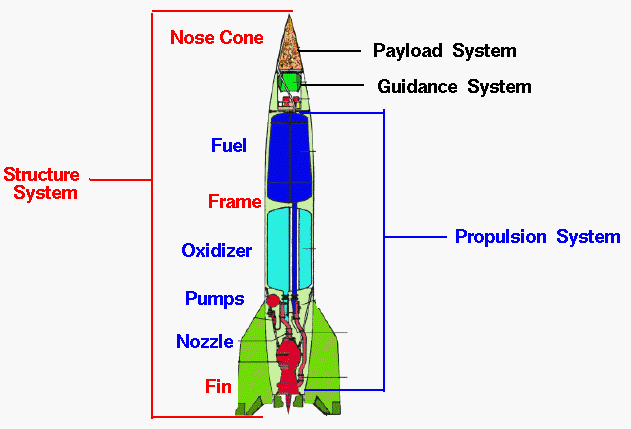
\includegraphics[width=0.6\textwidth]{figures/RocketStructure.png} 
 	\caption{Basic structure of a rocket.}
 	\label{fig:RocketStructure}
\end{figure}
%https://spaceflightsystems.grc.nasa.gov/education/rocket/rockpart.html


\section{Stability of a Rocket}
Describe why stability is important for a rocket. 
\section{Mechanical System of a Rocket}
Input/output relation of a rocket.
\section{The Inverse Pendulum}
relate the rocket model to a Inverse Pendulum